In this page the professor can see its scheduled meetings and cancel them.\\
The professor can either:
\begin{itemize}
    \item Delete a meeting: by clicking on the corresponding button 
    \item change month of the shown meetings: by clicking on the buttons placed under the meetings list 
\end{itemize}
\begin{figure}[H]
    \centering
    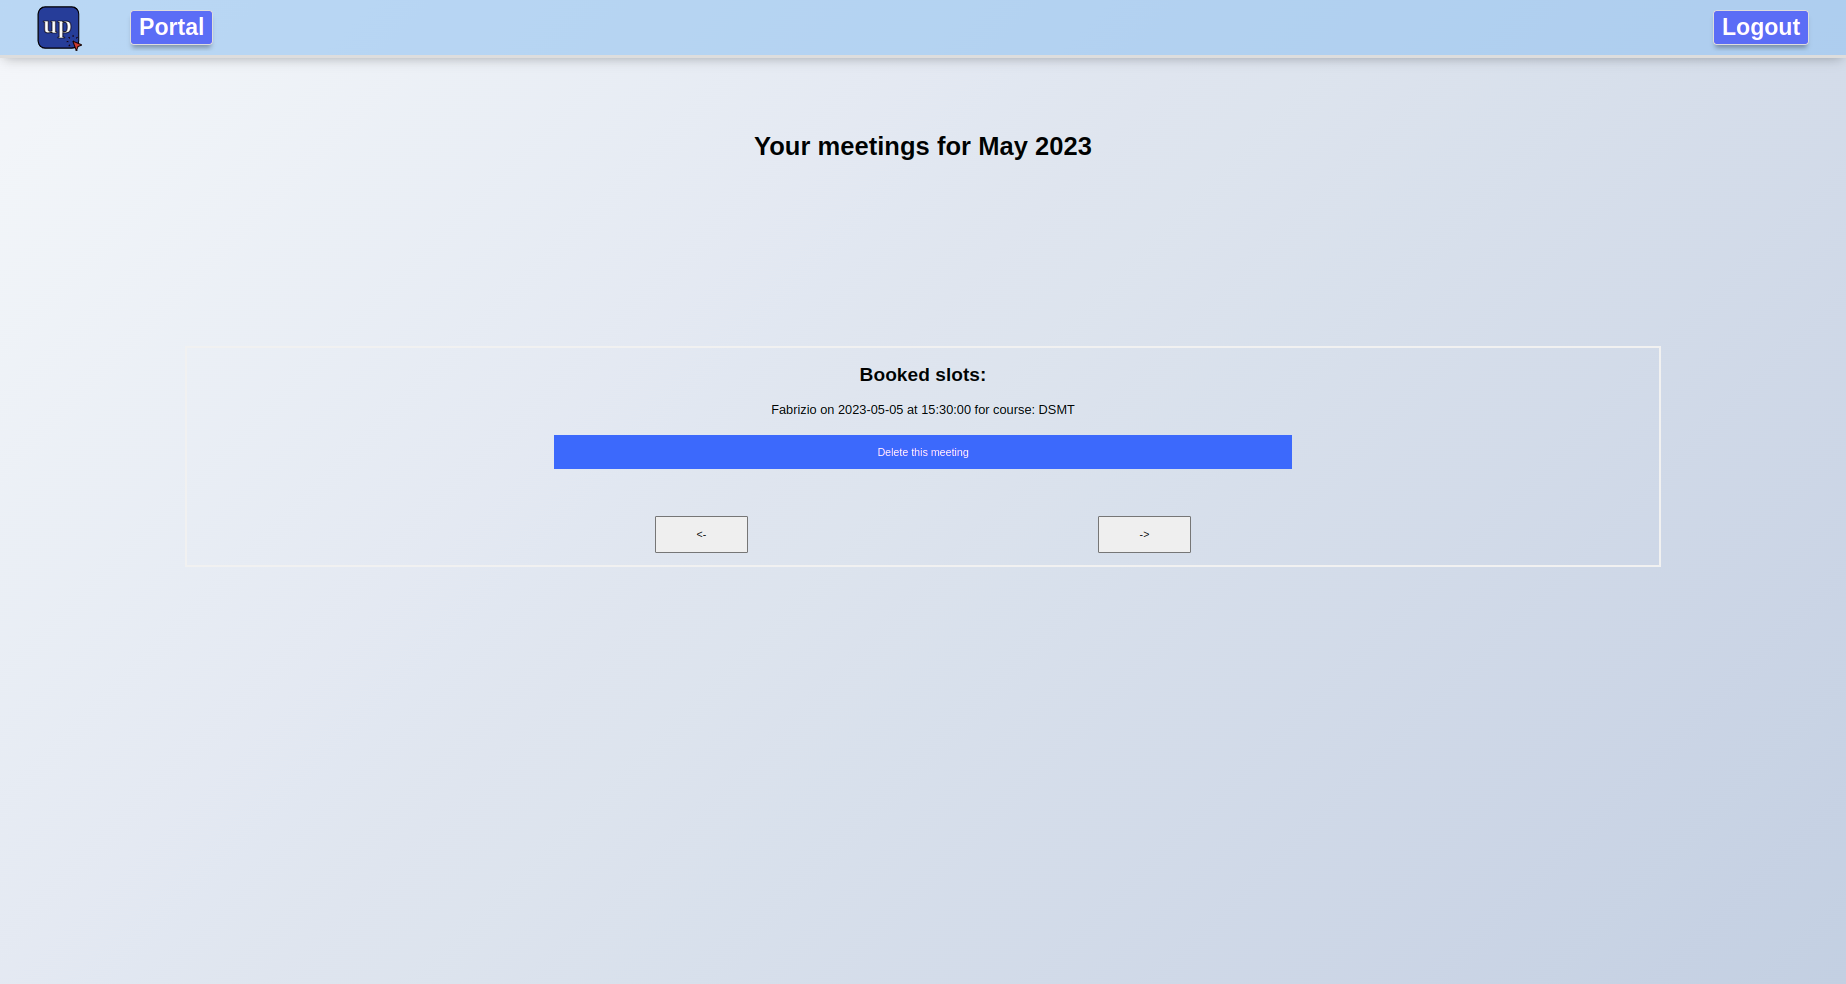
\includegraphics[width=\textwidth]{img/user_manual/professor/Meetings.png}
    \caption{Screenshot of professor/meeting page}
\end{figure}

After the deletion of a meeting the page will show an alert with the operation result.
\begin{figure}[H]
    \centering
    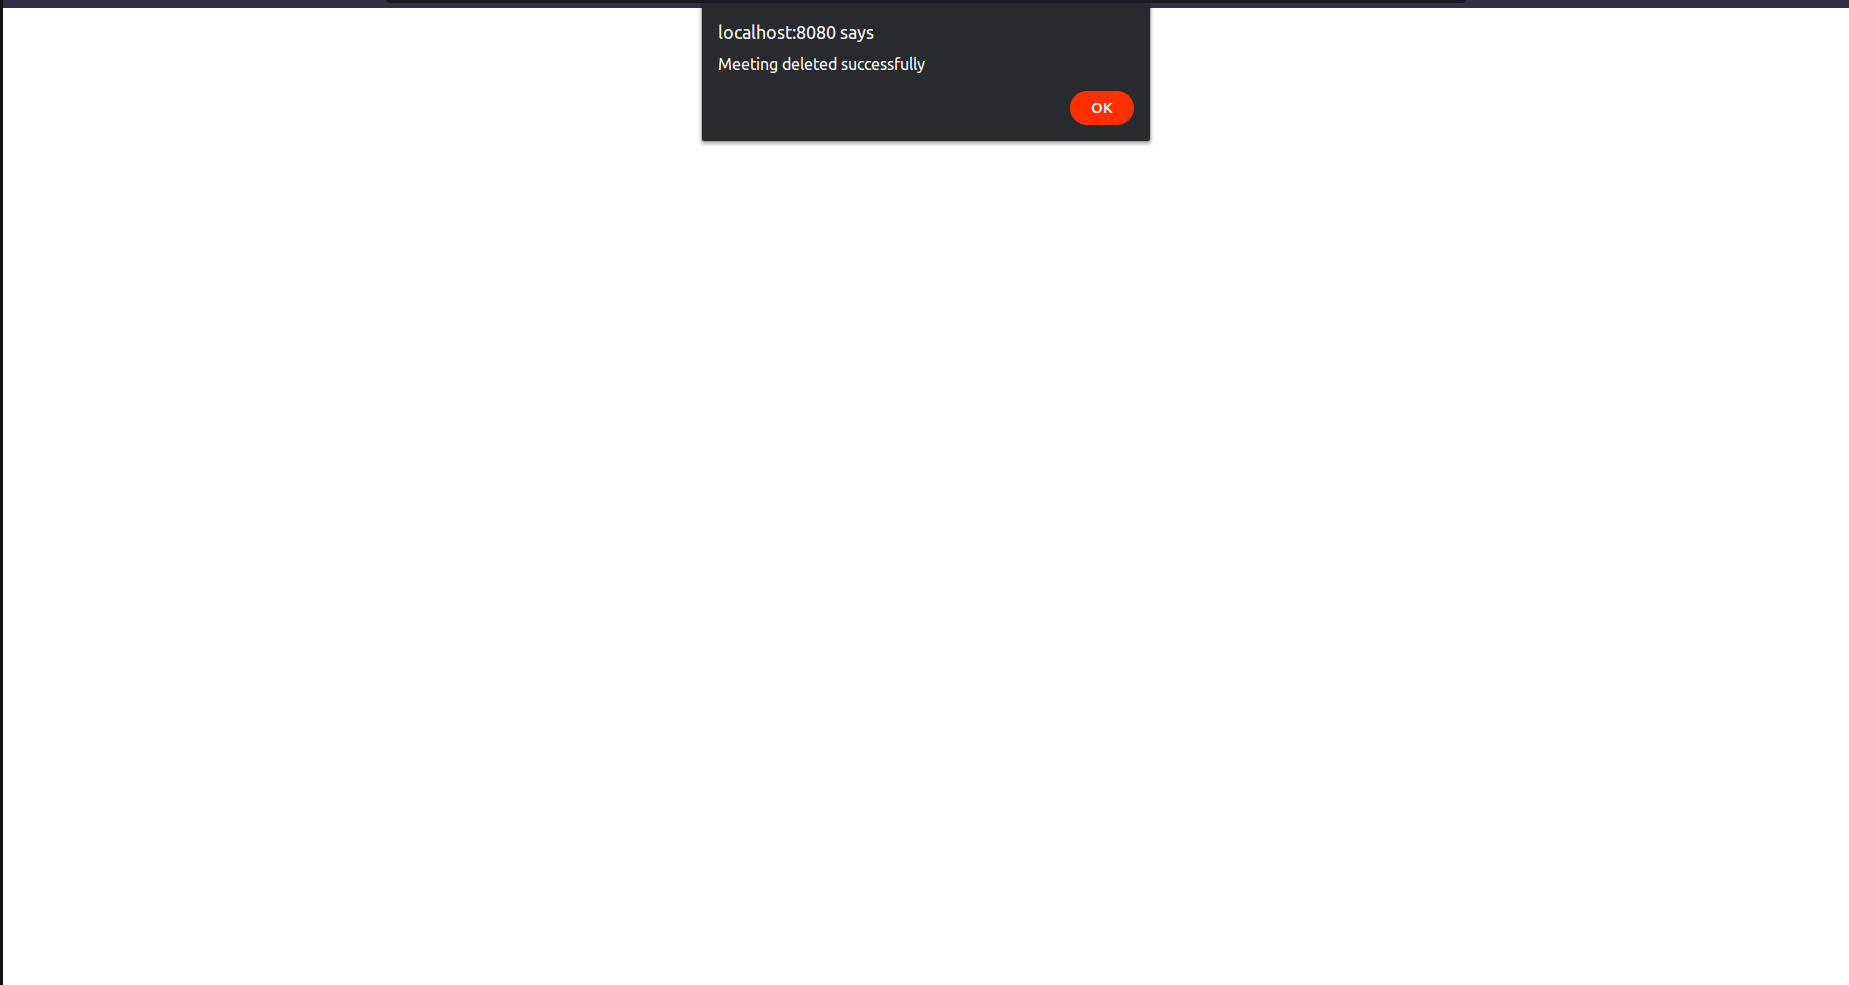
\includegraphics[width=\textwidth]{img/user_manual/professor/meeting-response.png}
    \caption{Screenshot of meeting deletion response}
\end{figure}